\documentclass[12pt,a4paper]{amsart}

\usepackage[T1]{fontenc}
\usepackage[utf8]{inputenc}
\usepackage[english]{babel}
\usepackage{amsmath,amssymb,amsthm}
\usepackage{mathtools}
\usepackage{tikz}
\usepackage{geometry}
\usepackage[hidelinks]{hyperref}
\usetikzlibrary{arrows.meta,calc,fit,positioning,decorations.pathreplacing}
\geometry{margin=2.5cm}

\theoremstyle{definition}
\newtheorem{definition}{Definition}[section]
\newtheorem{notation}[definition]{Notation}

\theoremstyle{plain}
\newtheorem{lemma}[definition]{Lemma}
\newtheorem{observation}[definition]{Observation}
\newtheorem{proposition}[definition]{Proposition}
\newtheorem{theorem}[definition]{Theorem}

\newcommand{\len}[1]{\ell(#1)}
\newcommand{\dist}[3]{d_{#1}(#2,#3)}

\title{\textbf{On the size of semi-cutting sets in graphs}}
\author{}
\date{}

\begin{document}

\begin{abstract}
Let $G=(V,E)$ be a finite simple undirected graph. For $T\subseteq V$ and $F\subseteq E$, we call $F$ a semi-cutting set for $T$ if $\dist{G}{u}{w}<\dist{G\setminus F}{u}{w}$ for every pair of distinct terminals $u,w\in T$, where disconnected pairs have distance $\infty$. We prove that every such set satisfies $|F|\ge |T|-1$. The proof uses a shortest-path characterization of the semi-cutting property, its preservation under contracting the closed neighborhood of a terminal not incident to $F$, and a lexicographic induction on the pair $(|T|,|V|)$.
\end{abstract}

\maketitle

\section{Introduction}

Throughout the paper, graphs are finite, simple, and undirected. For a graph $G=(V,E)$, a terminal set $T\subseteq V$, and an edge set $F\subseteq E$, we say that $F$ is \emph{semi-cutting} for $T$ if $\dist{G}{u}{w}<\dist{G\setminus F}{u}{w}$ for every two distinct vertices $u,w\in T$. Distances are allowed to take the value $\infty$, so terminal pairs may become disconnected after deleting $F$. On the other hand, if $\dist{G}{u}{w}=\infty$ already in $G$, then the defining inequality would read $\infty<\infty$, which is impossible. Thus the statement concerns arbitrary simple graphs, but every actual instance with a semi-cutting set has all terminal pairs joined by paths in the original graph.

Semi-cutting sets lie between two classical edge-deletion themes. The multiterminal cut problem of Dahlhaus, Johnson, Papadimitriou, Seymour, and Yannakakis~\cite{dahlhaus1994} asks for the complete pairwise separation of the terminals. On instances in which all terminal pairs are connected in the original graph, every multiterminal cut is therefore semi-cutting, but the converse fails because a semi-cutting set may leave some terminal pairs connected while merely forcing their distances to increase. At the other end, the most-vital-link framework introduced by Corley and Sha~\cite{corley-sha} and refined in later work~\cite{malik-mittal-gupta,nardelli-proietti-widmayer} focuses on a single distinguished pair of vertices and studies deletions that enlarge the distance between them. Semi-cutting sets retain this geodesic viewpoint, but require it simultaneously for every pair of terminals.

The main result is the lower bound $|F|\ge |T|-1$ for every semi-cutting set. The proof has three structural ingredients. First, semi-cutting sets can be characterized by the requirement that they intersect every shortest path between distinct terminals. Second, if a terminal $t$ is not incident to any edge of $F$, then after contracting the closed neighborhood $N[t]$ to a single vertex, the resulting image of $F$ is still semi-cutting for the modified terminal set. Third, these two facts feed a lexicographic induction on $(|T|,|V|)$.

The bound is sharp. For every $k\ge 2$, let $G$ be the path with vertex set $\{v_0,v_1,\dots,v_{2k-2}\}$ and edge set $\bigl\{\{v_i,v_{i+1}\}: i=0,\dots,2k-3\bigr\}$. If $T=\{v_0,v_2,\dots,v_{2k-2}\}$ and $F=\bigl\{\{v_{2i},v_{2i+1}\}: i=0,\dots,k-2\bigr\}$, then $|F|=|T|-1$. After deleting $F$, each connected component contains exactly one terminal, so all terminal-terminal distances increase from finite values to $\infty$. Figure~\ref{fig:semi-cut-example} shows the case $k=3$.

\begin{figure}[htbp]
\centering
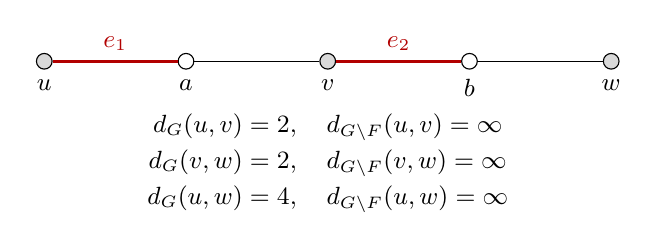
\begin{tikzpicture}[scale=1, every node/.style={font=\small}]
  \node[circle,draw,inner sep=2pt,fill=gray!30,label=below:$u$] (u) at (0,0) {};
  \node[circle,draw,inner sep=2pt,fill=white,label=below:$a$]   (a) at (1.8,0) {};
  \node[circle,draw,inner sep=2pt,fill=gray!30,label=below:$v$] (v) at (3.6,0) {};
  \node[circle,draw,inner sep=2pt,fill=white,label=below:$b$]   (b) at (5.4,0) {};
  \node[circle,draw,inner sep=2pt,fill=gray!30,label=below:$w$] (w) at (7.2,0) {};
  \draw[very thick,red!70!black] (u) -- node[above]{$e_1$} (a);
  \draw (a) -- (v);
  \draw[very thick,red!70!black] (v) -- node[above]{$e_2$} (b);
  \draw (b) -- (w);
  \node[align=center] at (3.6,-1.3)
    {$\dist{G}{u}{v}=2,\quad \dist{G\setminus F}{u}{v}=\infty$\\[2pt]
     $\dist{G}{v}{w}=2,\quad \dist{G\setminus F}{v}{w}=\infty$\\[2pt]
     $\dist{G}{u}{w}=4,\quad \dist{G\setminus F}{u}{w}=\infty$};
\end{tikzpicture}
\caption{A sharp example with $T=\{u,v,w\}$ and $F=\{e_1,e_2\}$.}
\label{fig:semi-cut-example}
\end{figure}

\section{Preliminaries}

Let $G=(V,E)$ be a finite simple graph. Distances take values in $\mathbb{N}_0\cup\{\infty\}$, ordered by $n<\infty$ for every $n\in\mathbb{N}_0$.

\begin{definition}[Walks, paths, and distance]\label{def:paths-distance}
Let $u,w\in V$. A walk from $u$ to $w$ is a sequence $P=(v_0,v_1,\dots,v_k)$, where $k\in\mathbb{N}_0$, $v_0=u$, $v_k=w$, and $\{v_{i-1},v_i\}\in E$ for every $i\in\{1,\dots,k\}$. Its length is $\len{P}\coloneqq k$. A path is a walk with pairwise distinct vertices. For a path $P=(v_0,\dots,v_k)$, we write $V(P)\coloneqq \{v_0,\dots,v_k\}$ and $E(P)\coloneqq \bigl\{\{v_{i-1},v_i\}: i=1,\dots,k\bigr\}$.

The distance $\dist{G}{u}{w}$ is the minimum length of a path from $u$ to $w$ in $G$ when such a path exists, and $\infty$ otherwise. A path $P$ from $u$ to $w$ is \emph{shortest} if $\len{P}=\dist{G}{u}{w}$.
\end{definition}

\begin{notation}[Basic graph operations]\label{not:basic-operations}
If $F\subseteq E$, then $G\setminus F$ denotes the graph $(V,E\setminus F)$, and $V[F]\coloneqq \{v\in V:\ \exists\, e\in F \text{ with } v\in e\}$ is the set of endpoints of the edges in $F$. For a vertex $v\in V$, its open and closed neighborhoods are $N(v)\coloneqq \{w\in V:\ \{v,w\}\in E\}$ and $N[v]\coloneqq N(v)\cup\{v\}$. If $P=(v_0,\dots,v_k)$ is a path and $0\le i\le j\le k$, then $P[v_i,v_j]\coloneqq (v_i,\dots,v_j)$.
\end{notation}

\begin{definition}[Contraction of a non-empty vertex set]\label{def:contraction}
Let $\emptyset\neq W\subseteq V$ and let $w^\ast\notin V$ be a new vertex. Define $\pi_W\colon V\to (V\setminus W)\cup\{w^\ast\}$ by $\pi_W(v)=w^\ast$ for $v\in W$ and $\pi_W(v)=v$ for $v\notin W$. The graph $G/W$ is the simple graph with vertex set $(V\setminus W)\cup\{w^\ast\}$ and edge set
\[
E(G/W)=\bigl\{\{\pi_W(x),\pi_W(y)\}: \{x,y\}\in E,\ \pi_W(x)\neq \pi_W(y)\bigr\}.
\]
Thus edges whose endpoints both lie in $W$ disappear, while parallel edges are identified automatically because the edge set consists of two-element subsets. If $e=\{x,y\}\in E$ and $\pi_W(x)\neq \pi_W(y)$, we write $e/W\coloneqq \{\pi_W(x),\pi_W(y)\}\in E(G/W)$. For $F\subseteq E$, we also put $F/W\coloneqq \bigl\{\{\pi_W(x),\pi_W(y)\}: \{x,y\}\in F,\ \pi_W(x)\neq \pi_W(y)\bigr\}\subseteq E(G/W)$.
\end{definition}

\begin{figure}[ht]
\centering
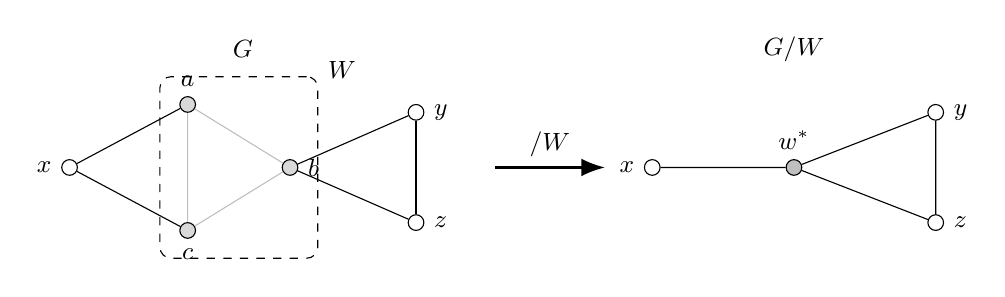
\begin{tikzpicture}[scale=1.0, every node/.style={font=\small}]
  \begin{scope}[xshift=0cm]
    \node at (2.2,3.0) {$G$};
    \node[circle,draw,inner sep=2pt,fill=white,label=left:$x$]    (x)  at (0,1.5)   {};
    \node[circle,draw,inner sep=2pt,fill=white,label=right:$y$]   (y)  at (4.4,2.2)  {};
    \node[circle,draw,inner sep=2pt,fill=white,label=right:$z$]   (z)  at (4.4,0.8)  {};
    \node[circle,draw,inner sep=2pt,fill=gray!30,label=above:$a$] (a)  at (1.5,2.3)  {};
    \node[circle,draw,inner sep=2pt,fill=gray!30,label=right:$b$] (b)  at (2.8,1.5)  {};
    \node[circle,draw,inner sep=2pt,fill=gray!30,label=below:$c$] (c)  at (1.5,0.7)  {};
    \draw[gray!50] (a)--(b)--(c)--(a);
    \draw (x)--(a)  (x)--(c);
    \draw (b)--(y)  (b)--(z);
    \draw (y)--(z);
    \node[draw,dashed,rounded corners,fit=(a)(b)(c),inner sep=7pt,
          label={[font=\small]above right:$W$}] {};
  \end{scope}
  \draw[-{Latex[length=3mm]},thick] (5.4,1.5) -- (6.8,1.5)
    node[midway,above,font=\small] {$/W$};
  \begin{scope}[xshift=7.4cm]
    \node at (1.8,3.0) {$G/W$};
    \node[circle,draw,inner sep=2pt,fill=white,label=left:$x$]       (xp) at (0,1.5)   {};
    \node[circle,draw,inner sep=2pt,fill=white,label=right:$y$]      (yp) at (3.6,2.2)  {};
    \node[circle,draw,inner sep=2pt,fill=white,label=right:$z$]      (zp) at (3.6,0.8)  {};
    \node[circle,draw,inner sep=2pt,fill=gray!50,label=above:$w^*$]  (wp) at (1.8,1.5)  {};
    \draw (xp)--(wp)  (wp)--(yp)  (wp)--(zp)  (yp)--(zp);
  \end{scope}
\end{tikzpicture}
\caption{Contracting $W=\{a,b,c\}$ to the vertex $w^\ast$.}
\label{fig:contraction-def}
\end{figure}

\begin{definition}[Semi-cutting set]\label{def:semi-cut}
Let $T\subseteq V$. An edge set $F\subseteq E$ is a \emph{semi-cutting set} for $T$ in $G$ if $\dist{G}{u}{w}<\dist{G\setminus F}{u}{w}$ for every pair of distinct vertices $u,w\in T$. The vertices of $T$ are the \emph{terminals}.
\end{definition}

\begin{observation}\label{obs:finite-terminal-distances}
If $F$ is a semi-cutting set for $T$ in $G$, then $\dist{G}{u}{w}<\infty$ for all distinct terminals $u,w\in T$.
\end{observation}

\begin{proof}
If $\dist{G}{u}{w}=\infty$ for some distinct $u,w\in T$, then Definition~\ref{def:semi-cut} would give $\infty=\dist{G}{u}{w}<\dist{G\setminus F}{u}{w}\le \infty$, a contradiction.
\end{proof}

\begin{observation}\label{obs:shortest-paths}
Let $X\subseteq V$ and $M\subseteq E$. Then $M$ is a semi-cutting set for $X$ in $G$ if and only if two conditions hold for every distinct $u,w\in X$: first, $\dist{G}{u}{w}<\infty$; second, every shortest $u$--$w$ path in $G$ contains an edge of $M$.
\end{observation}

\begin{proof}
Assume first that $M$ is semi-cutting for $X$. Observation~\ref{obs:finite-terminal-distances} gives $\dist{G}{u}{w}<\infty$. Let $P$ be a shortest $u$--$w$ path in $G$. If $E(P)\cap M=\emptyset$, then $P$ is also a path in $G\setminus M$, so $\dist{G\setminus M}{u}{w}\le \len{P}=\dist{G}{u}{w}$, contradicting Definition~\ref{def:semi-cut}.

Conversely, assume that for every distinct $u,w\in X$ the distance $\dist{G}{u}{w}$ is finite and every shortest $u$--$w$ path in $G$ meets $M$. Fix such a pair $u,w$. If $u$ and $w$ are disconnected in $G\setminus M$, then $\dist{G\setminus M}{u}{w}=\infty>\dist{G}{u}{w}$. Otherwise let $Q$ be a shortest $u$--$w$ path in $G\setminus M$. Then $Q$ is also a path in $G$, hence $\len{Q}\ge \dist{G}{u}{w}$. Equality is impossible, because then $Q$ would be a shortest $u$--$w$ path in $G$ disjoint from $M$. Therefore $\dist{G\setminus M}{u}{w}=\len{Q}>\dist{G}{u}{w}$, and $M$ is semi-cutting for $X$.
\end{proof}

\begin{figure}[ht]
\centering
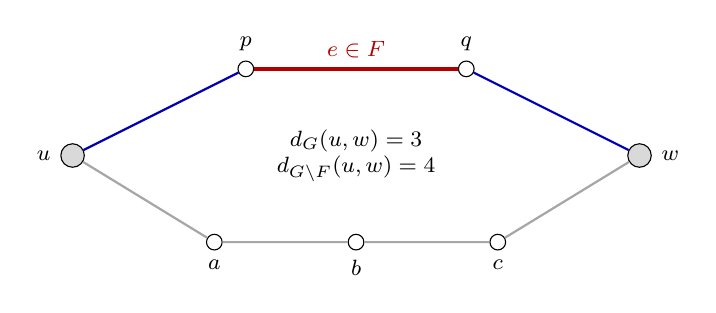
\begin{tikzpicture}[scale=1.0, every node/.style={font=\footnotesize}]
  \node[circle,draw,inner sep=3pt,fill=gray!30,label=left:$u$]  (u) at (0,0)   {};
  \node[circle,draw,inner sep=3pt,fill=gray!30,label=right:$w$] (w) at (7.2,0) {};
  \node[circle,draw,inner sep=2pt,fill=white,label=above:$p$] (p) at (2.2,1.1) {};
  \node[circle,draw,inner sep=2pt,fill=white,label=above:$q$] (q) at (5.0,1.1) {};
  \draw[thick,blue!70!black] (u)--(p);
  \draw[very thick,red!70!black] (p)--node[above]{$e\in F$}(q);
  \draw[thick,blue!70!black] (q)--(w);
  \node[circle,draw,inner sep=2pt,fill=white,label=below:$a$] (a) at (1.8,-1.1) {};
  \node[circle,draw,inner sep=2pt,fill=white,label=below:$b$] (b) at (3.6,-1.1) {};
  \node[circle,draw,inner sep=2pt,fill=white,label=below:$c$] (c) at (5.4,-1.1) {};
  \draw[thick,black!35] (u)--(a)--(b)--(c)--(w);
  \node[align=center] at (3.6,0)
    {$\dist{G}{u}{w}=3$\\$\dist{G\setminus F}{u}{w}=4$};
\end{tikzpicture}
\caption{Every shortest $u$--$w$ path meets $F$, although longer ones may avoid it.}
\label{fig:shortest-path-condition}
\end{figure}

\section{Preservation Under Contraction}

We use two standard facts on shortest paths without separate proof: every walk contains a path between the same endpoints whose length is no larger, and every subpath of a shortest path is shortest between its own endpoints; see, for example, Diestel~\cite[Chapter~1]{diestel}.

\begin{lemma}\label{lem:contraction-image-size}
Let $\emptyset\neq W\subseteq V$ and $F\subseteq E$. Then $|F/W|\le |F|$.
\end{lemma}

\begin{proof}
Let $D\coloneqq \bigl\{e\in F:\ e/W \text{ is defined}\bigr\}$. The map $D\to F/W$, given by $e\mapsto e/W$, is surjective, hence $|F/W|\le |D|\le |F|$.
\end{proof}

\begin{lemma}\label{lem:projection-walk}
Let $\emptyset\neq W\subseteq V$. If $P=(v_0,\dots,v_k)$ is a walk in $G$, then $G/W$ contains a walk $P'=(w_0,\dots,w_m)$ with $w_0=\pi_W(v_0)$, $w_m=\pi_W(v_k)$, and $m\le k$.
\end{lemma}

\begin{proof}
Start from the sequence $\bigl(\pi_W(v_0),\dots,\pi_W(v_k)\bigr)$ and delete every term equal to its immediate predecessor. The resulting sequence $P'=(w_0,\dots,w_m)$ clearly satisfies $w_0=\pi_W(v_0)$, $w_m=\pi_W(v_k)$, and $m\le k$. If $w_r,w_{r+1}$ are consecutive terms of $P'$, then for some index $j\in\{1,\dots,k\}$ we have $w_r=\pi_W(v_{j-1})$, $w_{r+1}=\pi_W(v_j)$, and $\pi_W(v_{j-1})\neq \pi_W(v_j)$. Since $\{v_{j-1},v_j\}\in E(G)$, Definition~\ref{def:contraction} yields $\{w_r,w_{r+1}\}\in E(G/W)$. Hence $P'$ is a walk in $G/W$.
\end{proof}

\begin{figure}[ht]
\centering
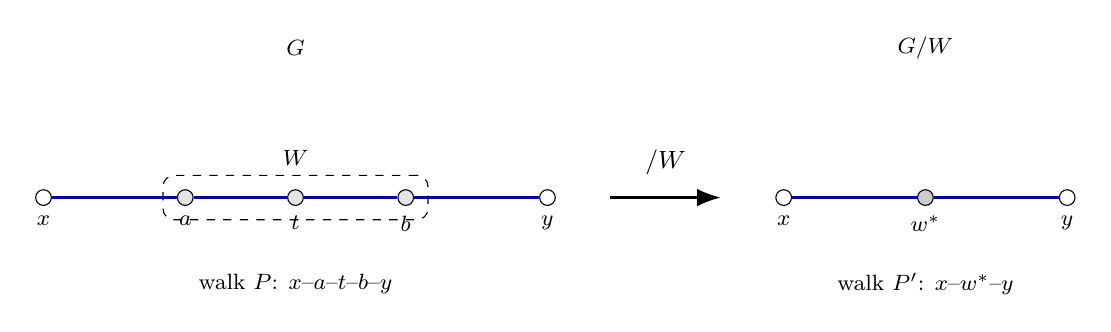
\begin{tikzpicture}[scale=1, every node/.style={font=\footnotesize}]
  \begin{scope}[xshift=0cm]
    \node[circle,draw,inner sep=2pt,fill=white,label=below:$x$]  (x)  at (0,0) {};
    \node[circle,draw,inner sep=2pt,fill=gray!20,label=below:$a$] (a)  at (1.8,0) {};
    \node[circle,draw,inner sep=2pt,fill=gray!20,label=below:$t$] (t)  at (3.2,0) {};
    \node[circle,draw,inner sep=2pt,fill=gray!20,label=below:$b$] (b)  at (4.6,0) {};
    \node[circle,draw,inner sep=2pt,fill=white,label=below:$y$]  (y)  at (6.4,0) {};
    \draw[very thick,blue!70!black] (x)--(a)--(t)--(b)--(y);
    \node[draw,dashed,rounded corners,fit=(a)(t)(b),inner sep=5pt,label=above:$W$] {};
    \node at (3.2,-1.1) {walk $P$: $x$--$a$--$t$--$b$--$y$};
    \node at (3.2,1.9) {$G$};
  \end{scope}
  \draw[-{Latex[length=3mm]},thick] (7.2,0) -- (8.6,0);
  \node at (7.9,0.45) {\small $/W$};
  \begin{scope}[xshift=9.4cm]
    \node[circle,draw,inner sep=2pt,fill=white,label=below:$x$]     (xp) at (0,0) {};
    \node[circle,draw,inner sep=2pt,fill=gray!40,label=below:$w^*$] (wp) at (1.8,0) {};
    \node[circle,draw,inner sep=2pt,fill=white,label=below:$y$]     (yp) at (3.6,0) {};
    \draw[very thick,blue!70!black] (xp)--(wp)--(yp);
    \node at (1.8,-1.1) {walk $P'$: $x$--$w^*$--$y$};
    \node at (1.8,1.9) {$G/W$};
  \end{scope}
\end{tikzpicture}
\caption{Projecting a walk under contraction can only shorten it.}
\label{fig:projection-walk}
\end{figure}

\begin{lemma}\label{lem:lifting-endpoint}
Let $t\in V$, let $t^\prime\notin V$ be a new vertex, and let $G^\prime\coloneqq G/N[t]$. Let $z\in V\setminus N[t]$, and let $P^\prime=(t^\prime,x_1,\dots,x_k)$ be a shortest path from $t^\prime$ to $z$ in $G^\prime$. Then there exists a vertex $v\in N(t)$ such that $P=(t,v,x_1,\dots,x_k)$ is a shortest path from $t$ to $z$ in $G$.
\end{lemma}

\begin{proof}
Since $z\neq t^\prime$, we have $k\ge 1$. The edge $\{t^\prime,x_1\}$ belongs to $E(G^\prime)$, so Definition~\ref{def:contraction} provides a vertex $v\in N[t]$ with $\{v,x_1\}\in E(G)$. Because $x_1\notin N[t]$, the choice $v=t$ is impossible, hence $v\in N(t)$. Every vertex $x_i$ lies outside $N[t]$, and the edges $\{x_{i-1},x_i\}$ of $P^\prime$ are therefore also edges of $G$. Consequently $P=(t,v,x_1,\dots,x_k)$ is a path in $G$ and $\len{P}=\len{P^\prime}+1$.

Now let $Q=(q_0,\dots,q_\ell)$ be any path from $t$ to $z$ in $G$. Since $z\notin N[t]$, the path has length at least $2$, so $q_1\in N(t)\subseteq N[t]$. Apply Lemma~\ref{lem:projection-walk} to the final segment $(q_1,\dots,q_\ell)$. This yields a walk from $t^\prime$ to $z$ in $G^\prime$ of length at most $\ell-1$, hence a path from $t^\prime$ to $z$ of length at most $\ell-1$ by the standard path-extraction fact quoted above. Therefore $\dist{G^\prime}{t^\prime}{z}\le \ell-1=\len{Q}-1$. Since $Q$ was arbitrary, $\dist{G}{t}{z}\ge \dist{G^\prime}{t^\prime}{z}+1$. On the other hand, $P$ is a $t$--$z$ path in $G$, so
\[
\dist{G}{t}{z}\le \len{P}=\len{P^\prime}+1=\dist{G^\prime}{t^\prime}{z}+1.
\]
The two inequalities give $\dist{G}{t}{z}=\len{P}$, and $P$ is shortest.
\end{proof}

\begin{observation}\label{obs:outside-edges}
Let $t\in V$, let $t^\prime\notin V$ be a new vertex, and let $G^\prime\coloneqq G/N[t]$. If $x,y\in V\setminus N[t]$ are distinct, then $\{x,y\}\in E(G^\prime)$ if and only if $\{x,y\}\in E(G)$; in that case $\{x,y\}/N[t]=\{x,y\}$.
\end{observation}

\begin{proof}
If $\{x,y\}\in E(G)$, then Definition~\ref{def:contraction} gives $\{x,y\}\in E(G^\prime)$ and $\{x,y\}/N[t]=\{x,y\}$. Conversely, if $\{x,y\}\in E(G^\prime)$, then some edge $\{u,v\}\in E(G)$ satisfies $\{\pi_{N[t]}(u),\pi_{N[t]}(v)\}=\{x,y\}$. Since neither $x$ nor $y$ is $t^\prime$, both $u$ and $v$ lie outside $N[t]$, so $\{u,v\}=\{x,y\}\in E(G)$.
\end{proof}

\begin{figure}[t]
\centering
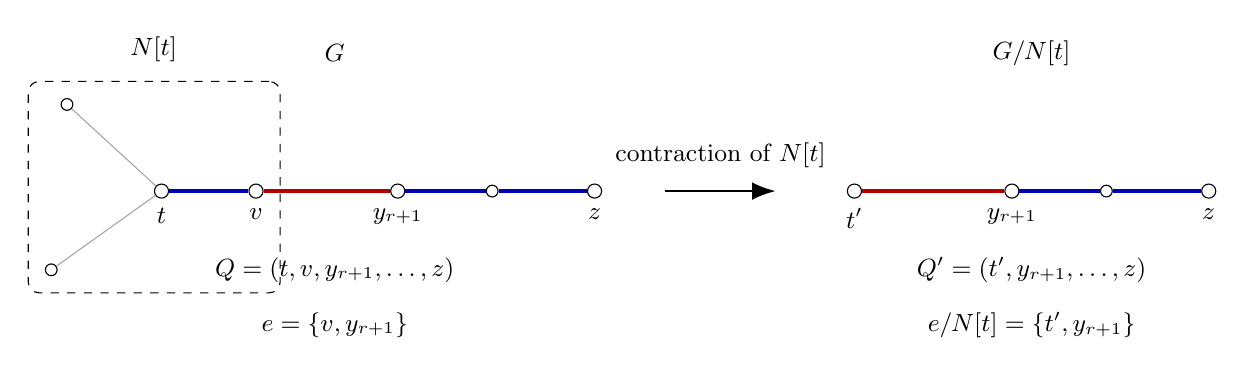
\begin{tikzpicture}[scale=1, every node/.style={font=\small}]
  \begin{scope}[xshift=0cm]
    \node[circle,draw,inner sep=1.5pt,fill=white] (a) at (-0.2,1.1) {};
    \node[circle,draw,inner sep=1.5pt,fill=white] (b) at (-0.4,-1.0) {};
    \node[circle,draw,inner sep=1.8pt,fill=white,label=below:$t$] (t) at (1.0,0.0) {};
    \node[circle,draw,inner sep=1.8pt,fill=white,label=below:$v$] (v) at (2.2,0.0) {};
    \node[circle,draw,inner sep=1.8pt,fill=white,label=below:$y_{r+1}$] (y1) at (4.0,0.0) {};
    \node[circle,draw,inner sep=1.5pt,fill=white] (y2) at (5.2,0.0) {};
    \node[circle,draw,inner sep=1.8pt,fill=white,label=below:$z$] (z) at (6.5,0.0) {};
    \draw[gray!70] (a)--(t) (b)--(t) (t)--(v);
    \draw[very thick,blue!70!black] (t)--(v)--(y1)--(y2)--(z);
    \draw[very thick,red!70!black] (v)--(y1);
    \node[draw,dashed,rounded corners,fit=(a)(b)(t)(v),inner sep=6pt] {};
    \node at (0.9,1.8) {$N[t]$};
    \node at (3.2,-1.0) {$Q=(t,v,y_{r+1},\dots,z)$};
    \node at (3.2,-1.7) {$e=\{v,y_{r+1}\}$};
    \node at (3.2,1.75) {$G$};
  \end{scope}

  \draw[-{Latex[length=3mm]},thick] (7.4,0) -- (8.8,0);
  \node at (8.1,0.45) {\small contraction of $N[t]$};

  \begin{scope}[xshift=9.8cm]
    \node[circle,draw,inner sep=1.8pt,fill=white,label=below:$t^\prime$] (tp) at (0.0,0.0) {};
    \node[circle,draw,inner sep=1.8pt,fill=white,label=below:$y_{r+1}$] (yp1) at (2.0,0.0) {};
    \node[circle,draw,inner sep=1.5pt,fill=white] (yp2) at (3.2,0.0) {};
    \node[circle,draw,inner sep=1.8pt,fill=white,label=below:$z$] (zp) at (4.5,0.0) {};
    \draw[very thick,blue!70!black] (tp)--(yp1)--(yp2)--(zp);
    \draw[very thick,red!70!black] (tp)--(yp1);
    \node at (2.25,-1.0) {$Q^\prime=(t^\prime,y_{r+1},\dots,z)$};
    \node at (2.25,-1.7) {$e/N[t]=\{t^\prime,y_{r+1}\}$};
    \node at (2.25,1.75) {$G/N[t]$};
  \end{scope}
\end{tikzpicture}
\caption{Lifting the final segment of a shortest path from $G/N[t]$ to $G$.}
\label{fig:contraction}
\end{figure}

\begin{proposition}\label{prop:contraction}
Let $T\subseteq V$ and $F\subseteq E$. Assume that $F$ is a semi-cutting set for $T$ in $G$. Let $t\in T\setminus V[F]$ and let $t^\prime\notin V$ be a new vertex. Put $G^\prime\coloneqq G/N[t]$, $T^\prime\coloneqq (T\setminus\{t\})\cup\{t^\prime\}$, and $F^\prime\coloneqq F/N[t]$. Then $F^\prime$ is a semi-cutting set for $T^\prime$ in $G^\prime$.
\end{proposition}

\begin{proof}
First, no terminal of $T\setminus\{t\}$ lies in $N[t]$. Indeed, if some $u\in T\setminus\{t\}$ were adjacent to $t$, then the unique shortest $t$--$u$ path would be the edge $\{t,u\}$. Observation~\ref{obs:shortest-paths} would force $\{t,u\}\in F$, contradicting $t\notin V[F]$. Hence $T\setminus\{t\}\subseteq V\setminus N[t]$, so $T^\prime\subseteq V(G^\prime)$.

Second, every pair of distinct terminals in $T^\prime$ has finite distance in $G^\prime$. If $u,w\in T\setminus\{t\}$, then Observation~\ref{obs:finite-terminal-distances} gives a $u$--$w$ path in $G$; its projection is a $u$--$w$ walk in $G^\prime$, hence a $u$--$w$ path. If one terminal is $t^\prime$ and the other is $z\in T\setminus\{t\}$, then a $t$--$z$ path in $G$ projects to a $t^\prime$--$z$ walk in $G^\prime$, and again to a path. Thus Observation~\ref{obs:shortest-paths} reduces the proof to showing that every shortest path between distinct terminals of $T^\prime$ intersects $F^\prime$.

Let $u,w\in T^\prime$ be distinct, and let $P^\prime$ be a shortest $u$--$w$ path in $G^\prime$.

\smallskip\noindent
\textbf{Case 1: $t^\prime\notin V(P^\prime)$.}
Then all vertices of $P^\prime$ lie in $V\setminus N[t]$, so Observation~\ref{obs:outside-edges} shows that $P^\prime$ is also a path in $G$. It is shortest there as well: otherwise a shorter $u$--$w$ path in $G$ would project to a $u$--$w$ walk in $G^\prime$ of no greater length, and therefore to a shorter $u$--$w$ path in $G^\prime$, impossible. Since $u,w\in T\setminus\{t\}$, Observation~\ref{obs:shortest-paths} yields an edge $g\in E(P^\prime)\cap F$. Again by Observation~\ref{obs:outside-edges}, $g/N[t]=g$, so $g\in F^\prime$.

\smallskip\noindent
\textbf{Case 2: $t^\prime\in V(P^\prime)$.}
Because the endpoints of $P^\prime$ play symmetric roles, we may index the path as $P^\prime=(y_0,\dots,y_m)$ with $y_r=t^\prime$ for some $r<m$. Set $z\coloneqq y_m\in T^\prime\setminus\{t^\prime\}=T\setminus\{t\}$ and $Q^\prime\coloneqq P^\prime[y_r,y_m]$. By the standard subpath property, $Q^\prime$ is a shortest path from $t^\prime$ to $z$ in $G^\prime$. Lemma~\ref{lem:lifting-endpoint} therefore gives a vertex $v\in N(t)$ such that $Q=(t,v,y_{r+1},\dots,y_m)$ is a shortest path from $t$ to $z$ in $G$.

Since $t,z\in T$, Observation~\ref{obs:shortest-paths} implies $E(Q)\cap F\neq\emptyset$. No edge of $F$ is incident to $t$, because $t\notin V[F]$, so the first edge $\{t,v\}$ of $Q$ does not belong to $F$. Choose $f\in E(Q)\cap F$. If $f=\{v,y_{r+1}\}$, then $f/N[t]=\{t^\prime,y_{r+1}\}$ is the first edge of $Q^\prime$. Otherwise $f=\{y_i,y_{i+1}\}$ for some $i\in\{r+1,\dots,m-1\}$, and both endpoints lie outside $N[t]$; hence Observation~\ref{obs:outside-edges} gives $f/N[t]=f\in E(Q^\prime)$. In both subcases, $f/N[t]\in E(Q^\prime)\subseteq E(P^\prime)$ and $f/N[t]\in F^\prime$.

Thus every shortest path between distinct terminals in $T^\prime$ meets $F^\prime$. Observation~\ref{obs:shortest-paths} completes the proof.
\end{proof}

\section{Main Theorem}

\begin{theorem}\label{thm:main}
Let $G=(V,E)$ be a finite simple undirected graph, let $T\subseteq V$, and let $F\subseteq E$. If $F$ is a semi-cutting set for $T$ in $G$, then $|F|\ge |T|-1$.
\end{theorem}

\begin{figure}[t]
\centering
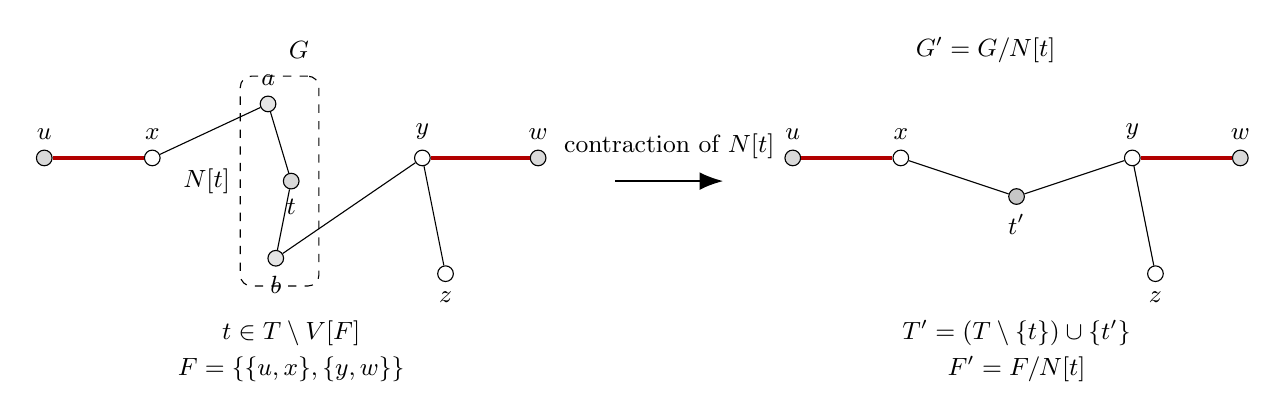
\begin{tikzpicture}[scale=0.98, every node/.style={font=\small}]
  \begin{scope}[xshift=0cm]
    \node at (3.3,2.9) {$G$};
    \node[circle,draw,inner sep=2pt,fill=gray!30,label=above:$u$] (u) at (0.0,1.5) {};
    \node[circle,draw,inner sep=2pt,fill=white,label=above:$x$] (x) at (1.4,1.5) {};
    \node[circle,draw,inner sep=2pt,fill=gray!20,label=above:$a$] (a) at (2.9,2.2) {};
    \node[circle,draw,inner sep=2pt,fill=gray!30,label=below:$t$] (t) at (3.2,1.2) {};
    \node[circle,draw,inner sep=2pt,fill=gray!20,label=below:$b$] (b) at (3.0,0.2) {};
    \node[circle,draw,inner sep=2pt,fill=white,label=above:$y$] (y) at (4.9,1.5) {};
    \node[circle,draw,inner sep=2pt,fill=gray!30,label=above:$w$] (w) at (6.4,1.5) {};
    \node[circle,draw,inner sep=2pt,fill=white,label=below:$z$] (z) at (5.2,0.0) {};
    \draw[very thick,red!70!black] (u)--(x);
    \draw (x)--(a)--(t)--(b)--(y);
    \draw[very thick,red!70!black] (y)--(w);
    \draw (y)--(z);
    \node[draw,dashed,rounded corners,fit=(a)(t)(b),inner sep=7pt,label=left:{$N[t]$}] {};
    \node[align=center] at (3.2,-1.0)
      {$t\in T\setminus V[F]$\\[2pt] $F=\{\{u,x\},\{y,w\}\}$};
  \end{scope}

  \draw[-{Latex[length=3mm]},thick] (7.4,1.2) -- (8.8,1.2);
  \node at (8.1,1.65) {\small contraction of $N[t]$};

  \begin{scope}[xshift=9.7cm]
    \node at (2.5,2.9) {$G^\prime=G/N[t]$};
    \node[circle,draw,inner sep=2pt,fill=gray!30,label=above:$u$] (up) at (0.0,1.5) {};
    \node[circle,draw,inner sep=2pt,fill=white,label=above:$x$] (xp) at (1.4,1.5) {};
    \node[circle,draw,inner sep=2pt,fill=gray!45,label=below:$t^\prime$] (tp) at (2.9,1.0) {};
    \node[circle,draw,inner sep=2pt,fill=white,label=above:$y$] (yp) at (4.4,1.5) {};
    \node[circle,draw,inner sep=2pt,fill=gray!30,label=above:$w$] (wp) at (5.8,1.5) {};
    \node[circle,draw,inner sep=2pt,fill=white,label=below:$z$] (zp) at (4.7,0.0) {};
    \draw[very thick,red!70!black] (up)--(xp);
    \draw (xp)--(tp)--(yp);
    \draw[very thick,red!70!black] (yp)--(wp);
    \draw (yp)--(zp);
    \node[align=center] at (2.9,-1.0)
      {$T^\prime=(T\setminus\{t\})\cup\{t^\prime\}$\\[2pt] $F^\prime=F/N[t]$};
  \end{scope}
\end{tikzpicture}
\caption{Case 1 of Theorem~\ref{thm:main}: contracting the closed neighborhood of a terminal outside $V[F]$.}
\label{fig:main-contraction}
\end{figure}

\begin{figure}[t]
\centering
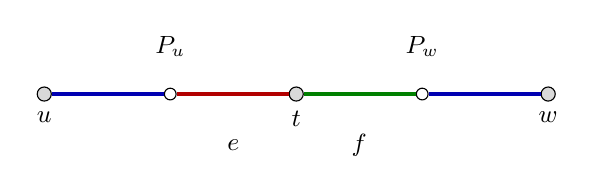
\begin{tikzpicture}[scale=1, every node/.style={font=\small}]
  \node[circle,draw,inner sep=1.8pt,fill=gray!30,label=below:$u$] (u) at (0,0) {};
  \node[circle,draw,inner sep=1.5pt,fill=white] (x) at (1.6,0) {};
  \node[circle,draw,inner sep=1.8pt,fill=gray!30,label=below:$t$] (t) at (3.2,0) {};
  \node[circle,draw,inner sep=1.5pt,fill=white] (y) at (4.8,0) {};
  \node[circle,draw,inner sep=1.8pt,fill=gray!30,label=below:$w$] (w) at (6.4,0) {};
  \draw[very thick,blue!70!black] (u)--(x)--(t)--(y)--(w);
  \draw[very thick,red!70!black] (x)--(t);
  \draw[very thick,green!50!black] (t)--(y);
  \node at (1.6,0.6) {$P_u$};
  \node at (4.8,0.6) {$P_w$};
  \node at (2.4,-0.65) {$e$};
  \node at (4.0,-0.65) {$f$};
\end{tikzpicture}
\caption{Case 2 of Theorem~\ref{thm:main}: splitting a shortest path at the removed terminal $t$.}
\label{fig:split-path}
\end{figure}

\begin{proof}
We prove the stronger statement that for every pair $(k,n)\in \mathbb{N}_0^2$, every simple graph $H$ on $n$ vertices, every set $X\subseteq V(H)$ of size $k$, and every edge set $M\subseteq E(H)$, if $M$ is semi-cutting for $X$ in $H$, then $|M|\ge k-1$. Order the relevant pairs lexicographically: $(k_1,n_1)\prec (k_2,n_2)$ when either $k_1<k_2$, or $k_1=k_2$ and $n_1<n_2$. This order is well-founded on $\{(a,b)\in\mathbb{N}_0^2:\ a\le b\}$, because every non-empty subset has a pair with minimal first coordinate and, among those, minimal second coordinate.

\smallskip\noindent
\textbf{Base case.}
If $k\le 1$, then there are no distinct terminal pairs, hence $|M|\ge 0\ge k-1$.

\smallskip\noindent
\textbf{Inductive step.}
Fix $(k,n)$ with $k\ge 2$, and assume the claim for every $(k',n')\prec (k,n)$. Let $G=(V,E)$ be a simple graph on $n$ vertices, let $T\subseteq V$ have size $k$, and let $F\subseteq E$ be semi-cutting for $T$ in $G$. We show $|F|\ge k-1$.

\smallskip\noindent
\textbf{Case 1: $T\setminus V[F]\neq \emptyset$.}
Choose $t\in T\setminus V[F]$. Since $k\ge 2$, there exists $u\in T\setminus\{t\}$. By Observation~\ref{obs:finite-terminal-distances}, the vertices $t$ and $u$ are joined by a path in $G$, so the first edge of such a path is incident to $t$. Hence $N(t)\neq\emptyset$, and therefore $|N[t]|\ge 2$. Let $t^\prime\notin V$ be a new vertex and define $G^\prime\coloneqq G/N[t]$, $T^\prime\coloneqq (T\setminus\{t\})\cup\{t^\prime\}$, and $F^\prime\coloneqq F/N[t]$, as in Figure~\ref{fig:main-contraction}. Proposition~\ref{prop:contraction} shows that $F^\prime$ is semi-cutting for $T^\prime$ in $G^\prime$. Moreover $|T^\prime|=|T|=k$ and
\[
|V(G^\prime)|=|V|-|N[t]|+1\le n-1<n.
\]
Thus $(|T^\prime|,|V(G^\prime)|)\prec (k,n)$, and the inductive hypothesis yields $|F^\prime|\ge |T^\prime|-1=k-1$. Lemma~\ref{lem:contraction-image-size} gives $|F^\prime|\le |F|$, so $|F|\ge k-1$.

\smallskip\noindent
\textbf{Case 2: $T\subseteq V[F]$.}
First note that $F\neq\emptyset$: if $F=\emptyset$, then $G\setminus F=G$, and Definition~\ref{def:semi-cut} would require $\dist{G}{u}{w}<\dist{G}{u}{w}$ for every distinct $u,w\in T$, impossible. Since $T\subseteq V[F]$, each terminal is incident to an edge of $F$. Choose $t\in T$ and an edge $e\in F$ incident to $t$, and set $T^-\coloneqq T\setminus\{t\}$ and $F^-\coloneqq F\setminus\{e\}$.

We claim that $F^-$ is semi-cutting for $T^-$ in $G$. By Observation~\ref{obs:finite-terminal-distances}, every pair of distinct vertices in $T^-$ has finite distance in $G$. It is therefore enough, by Observation~\ref{obs:shortest-paths}, to show that every shortest path between two distinct vertices of $T^-$ meets $F^-$.

Take distinct $u,w\in T^-$, and let $P$ be a shortest $u$--$w$ path in $G$. Since $u,w\in T$, Observation~\ref{obs:shortest-paths} gives $E(P)\cap F\neq\emptyset$. If $e\notin E(P)$, then already $E(P)\cap F^-\neq\emptyset$. Suppose now that $e\in E(P)$. Write $P=(v_0,\dots,v_m)$ and let $v_j=t$. Because $u,w\neq t$, we have $0<j<m$. Put $P_u\coloneqq (v_0,\dots,v_j)$ and $P_w\coloneqq (v_j,\dots,v_m)$, so Figure~\ref{fig:split-path} depicts the situation. By the standard subpath property, $P_u$ and $P_w$ are shortest paths for the pairs $(u,t)$ and $(t,w)$. Since $P$ is a path, the subpaths $P_u$ and $P_w$ share only the vertex $t$, so their edge sets are disjoint. As $e$ is incident to $t$, it belongs to exactly one of them.

If $e\in E(P_u)$, then $e\notin E(P_w)$. Because $t,w\in T$ and $P_w$ is a shortest $t$--$w$ path, Observation~\ref{obs:shortest-paths} yields an edge $f\in E(P_w)\cap F$. This edge satisfies $f\neq e$, hence $f\in F^-$. The case $e\in E(P_w)$ is symmetric, using the shortest path $P_u$ between $u$ and $t$. In either case, $E(P)\cap F^-\neq\emptyset$, and the claim follows.

Since $|T^-|=k-1$ and $|V(G)|=n$, we have $(|T^-|,|V(G)|)\prec (k,n)$. By the inductive hypothesis, $|F^-|\ge |T^-|-1=k-2$. Therefore $|F|=|F^-|+1\ge k-1$.
\end{proof}

\section{Concluding Remarks and Related Problems}

The path family from the introduction shows that Theorem~\ref{thm:main} is best possible. It would therefore be natural to characterize the extremal triples $(G,T,F)$ satisfying $|F|=|T|-1$.

The surrounding literature suggests two immediate directions. The multiterminal cut problem studied by Dahlhaus et al.~\cite{dahlhaus1994} asks for a minimum edge set whose deletion disconnects every terminal from every other one. On instances in which all terminal pairs are connected beforehand, this requirement is strictly stronger than semi-cutting: every multiterminal cut is semi-cutting, whereas a semi-cutting set may leave terminals connected and only force longer terminal-to-terminal geodesics. In contrast, the most-vital-edge line of work initiated by Corley and Sha~\cite{corley-sha} and continued in~\cite{malik-mittal-gupta,nardelli-proietti-widmayer} fixes a single pair of vertices and measures how much its distance can be increased by deletions. Semi-cutting sets preserve that distance-based viewpoint, but impose it simultaneously on all pairs in $T$.

This suggests, although it does not by itself prove, that optimization problems for semi-cutting sets may inherit part of the structural difficulty visible in multiterminal cuts. Weighted variants, vertex-deletion variants, and exact extremal descriptions for the equality case are natural next questions.

\begin{thebibliography}{7}

\bibitem{diestel}
R.~Diestel,
\emph{Graph Theory},
5th ed., Graduate Texts in Mathematics, vol.~173, Springer, Berlin, 2017.

\bibitem{corley-sha}
H.~W. Corley, D.~Y. Sha,
\emph{Most vital links and nodes in weighted networks},
Operations Research Letters 1(4) (1982), 157--160.

\bibitem{malik-mittal-gupta}
K.~Malik, A.~K. Mittal, S.~K. Gupta,
\emph{The $k$ most vital arcs in the shortest path problem},
Operations Research Letters 8(4) (1989), 223--227.

\bibitem{dahlhaus1994}
E.~Dahlhaus, D.~S. Johnson, C.~H. Papadimitriou, P.~D. Seymour, M.~Yannakakis,
\emph{The complexity of multiterminal cuts},
SIAM Journal on Computing 23(4) (1994), 864--894.

\bibitem{nardelli-proietti-widmayer}
E.~Nardelli, G.~Proietti, P.~Widmayer,
\emph{A faster computation of the most vital edge of a shortest path},
Information Processing Letters 79(2) (2001), 81--85.

\end{thebibliography}

\end{document}
